%               .-.
%              (o o)      SCIENCE OWL
%              | O \      (guardian of rigor)
%               \   \
%                `~~~'
%          .-------------------.
%          |  NO FABRICATION   |
%          |  + CLEAR ASSUMES  |
%          |  + CLEAN LATEX    |
%          '-------------------'
%     __        __        __        __
%  __/  \__  __/  \__  __/  \__  __/  \__
% /  RULES  \/  FLOW  \/  MATH  \/  CODE  \
% \__    __/\__    __/\__    __/\__    __/
%    \__/      \__/      \__/      \__/

%         \  |  /        \  |  /
%          \ | /          \ | /
%       ---- * ----    ---- * ----
%          / | \          / | \
%         /  |  \        /  |  \

%              ...                            
%             ;::::;                           
%           ;::::; :;                          
%         ;:::::'   :;                         
%        ;:::::;     ;.                        
%       ,:::::'       ;           OOO\         
%       ::::::;       ;          OOOOO\        
%       ;:::::;       ;         OOOOOOOO       
%      ,;::::::;     ;'         / OOOOOOO      
%    ;:::::::::`. ,,,;.        /  / DOOOOOO    
%  .';:::::::::::::::::;,     /  /     DOOOO   
% ,::::::;::::::;;;;::::;,   /  /        DOOO  
%;`::::::`'::::::;;;::::: ,#/  /          DOOO 
%:`:::::::`;::::::;;::: ;::#  /            DOOO
%::`:::::::`;:::::::: ;::::# /              DOO
%`:`:::::::`;:::::: ;::::::#/               DOO
% :::`:::::::`;; ;:::::::::##                OO
% ::::`:::::::`;::::::::;:::#                OO
% `:::::`::::::::::::;'`:;::#                O 
%  `:::::`::::::::;' /  / `:#                  
%   ::::::`:::::;'  /  /   `#              
%
%
%
%                           _,,,.._       ,_
%                        .gMMMMMMMMMp,_    `\
%                     .dMMP'       ``^YMb..dP
%                    dMMP'
%                    MMM:
%                    YMMb.
%                     YMMMb.
%                      `YMM/|Mb.  ,__
%                   _,,-~`--..-~-'_,/`--,,,____
%               `\,_,/',_.-~_..-~/' ,/---~~~"""`\
%          _,_,,,\q\q/'    \,,-~'_,/`````-,7.
%         `@v@`\\,,,,__   \,,-~~"__/` ",,/MMMMb.
%          `--''_..-~~\   \,-~~""  `\_,/ `^YMMMMMb..
%           ,|``-~~--./_,,_  _,,-~~'/_      `YMMMMMMMb.
%         ,/  `\,_,,/`\    `\,___,,,/M/'      `YMMMMMMMb
%                     ;  _,,/__...|MMM/         YMMMMMMMb
%                      .' /'      dMMM\         !MMMMMMMMb
%                   ,-'.-'""~~~--/M|M' \        !MMMMMMMMM
%                 ,/ .|...._____/MMM\   b       gMMMMMMMMM
%              ,'/'\/          dMMP/'   M.     ,MMMMMMMMMP
%             / `\;/~~~~----...MP'     ,MMb..,dMMMMMMMMM'
%            / ,_  |          _/      dMMMMMMMMMMMMMMMMB
%            \  |\,\,,,,___ _/    _,dMMMMMMMMMMMP".emmmb,
%             `.\  gY.     /      7MMMMMMMMMMP"..emmMMMMM
%                .dMMMb,-..|       `.~~"""```|dMMMMP'MMP'
%               .MMMMP^"""/ .7 ,  _  \,---~""`^YMMP'MM;
%             _dMMMP'   ,' / | |\ \\  }          PM^M^b
%          _,' _,  \_.._`./  } ; \ \``'      __,'_` _  `._
%      ,-~/'./'| 7`,,__,}`   ``   ``        // _/`| 7``-._`}
%     |_,}__{  {,/'   ``                    `\{_  {,/'   ``
%     ``  ```   ``                            ``   ``
%
%
%
%

% ----------------------------------------------------------
% CODE PRESENTATION
% ----------------------------------------------------------
% MATLAB code may be presented with full LaTeX formatting
% (listings / matlab-prettifier) for readability.
% Compact inline formatting is required ONLY when space
% constraints are explicitly stated.
% ==========================================================
% UNIVERSAL COURSEWORK TEMPLATE — v2.0 (SPECIFICATION-SAFE)
% Compile with XeLaTeX or LuaLaTeX (fontspec required)
% ==========================================================

\documentclass[11pt]{article}

% ----------------------------------------------------------
% ENGINE ASSUMPTION
% ----------------------------------------------------------
% This document MUST be compiled with XeLaTeX or LuaLaTeX.
% pdfLaTeX is not supported due to fontspec usage.

% ----------------------------------------------------------
% LANGUAGE & FONTS
% ----------------------------------------------------------
\usepackage[english]{babel}
\usepackage{csquotes}
\usepackage{fontspec}


% ----------------------------------------------------------
% PAGE LAYOUT
% ----------------------------------------------------------
\usepackage{geometry}
\geometry{
  a4paper,
  margin=20mm
}

\setlength{\parindent}{20pt}
\setlength{\parskip}{0.5em}

% ----------------------------------------------------------
% DEBUG / DRAFT TOGGLES
% ----------------------------------------------------------
\newif\ifshowlayout
\showlayoutfalse % set true for debugging

\ifshowlayout
  \usepackage{showframe}
\fi

% ----------------------------------------------------------
% MATHEMATICS
% ----------------------------------------------------------
\usepackage{amsmath, amssymb}
\usepackage{mathtools}
\numberwithin{equation}{section}
\usepackage{bigints}
\usepackage{siunitx}

\sisetup{
  detect-all,
  per-mode=symbol
}

% ----------------------------------------------------------
% FIGURES & TABLES
% ----------------------------------------------------------
\usepackage{graphicx}
\usepackage{float}
\usepackage{subcaption}
\usepackage{wrapfig}
\usepackage{longtable}
\usepackage{tabularx}
\usepackage{array}
\usepackage{multirow}
\usepackage{makecell}
\usepackage{booktabs}
\renewcommand{\arraystretch}{1.3}
\setlength{\tabcolsep}{10pt}

\usepackage{flafter}

% ----------------------------------------------------------
% COLOURS
% ----------------------------------------------------------
\usepackage[table]{xcolor}
\definecolor{babyblue}{RGB}{173,216,230}
\definecolor{BrightBlue}{RGB}{0,102,255}

% ----------------------------------------------------------
% TEXT & STRUCTURE
% ----------------------------------------------------------
\usepackage{ragged2e}
\usepackage{multicol}
\usepackage{titlesec}
\usepackage{titling}
\usepackage{layout}
\usepackage{todonotes}

\newcommand{\HRule}{\rule{\linewidth}{0.5mm}}

% ----------------------------------------------------------
% OPTIONAL: APPEND EXTERNAL PDFS
% ----------------------------------------------------------
% Uncomment ONLY if external PDFs must be appended
%
% \usepackage{pdfpages}
%
% Usage is controlled explicitly in the document body.


% ----------------------------------------------------------
% CODE (MINIMAL — STYLE GOVERNED BY RULESET)
% ----------------------------------------------------------
\usepackage{listings}
\usepackage{matlab-prettifier}

\lstset{
  basicstyle=\ttfamily\small,
  showstringspaces=false,
  breaklines=false
}

% ----------------------------------------------------------
% HEADERS & FOOTERS
% ----------------------------------------------------------
\usepackage{fancyhdr}
\pagestyle{fancy}
\fancyhead{}

\fancyfoot{}
\fancyfoot[CO]{\thepage}

% ----------------------------------------------------------
% BIBLIOGRAPHY
% ----------------------------------------------------------
\usepackage[
  backend=biber,
  style=numeric,
  sorting=none
]{biblatex}
\let\cite=\supercite%
\addbibresource{References/.bib}

\graphicspath{{Figures/}}
% ----------------------------------------------------------
% HYPERLINKS & REFERENCES
% ----------------------------------------------------------
\usepackage{xurl}
\usepackage{hyperref}
\usepackage{cleveref}

\hypersetup{
  breaklinks=true,
  colorlinks=true,
  linkcolor=BrightBlue,
  urlcolor=BrightBlue,
  citecolor=BrightBlue
}

% Full reference names (per ruleset)
\crefname{equation}{Equation}{Equations}
\crefname{figure}{Figure}{Figures}
\crefname{table}{Table}{Tables}
\crefname{section}{Section}{Sections}

% ----------------------------------------------------------
% CUSTOM COMMANDS
% ----------------------------------------------------------
\newcommand{\vect}[1]{\boldsymbol{#1}}
\newcommand{\dd}{\mathrm{d}}
\newcommand{\code}[1]{\texttt{#1}}
\newcommand{\data}[1]{\texttt{#1}}

% ----------------------------------------------------------
% SMART REFERENCE MACRO
% ----------------------------------------------------------
\usepackage{xstring}
\usepackage{etoolbox}

\newcommand{\smartref}[1]{%
  \IfSubStr{#1}{:}{%
    \StrBefore{#1}{:}[\RefPrefix]%
    \StrBehind{#1}{:}[\RefSuffix]%
    \ifdefstring{\RefPrefix}{fig}{Figure~\ref{#1}}{%
    \ifdefstring{\RefPrefix}{tab}{Table~\ref{#1}}{%
    \ifdefstring{\RefPrefix}{eq}{Equation~\ref{#1}}{%
    \ifdefstring{\RefPrefix}{sec}{Section~\ref{#1}}{%
      \ref{#1}%
    }}}}%
  }{%
    \ref{#1}%
  }%
}

% ----------------------------------------------------------
% TITLE INFORMATION
% ----------------------------------------------------------
\newcommand{\subtitle}[1]{%
  \posttitle{%
    \par\end{center}
    \begin{center}\large#1\end{center}
    \vskip0.5em}%
}
\fancyhead[RO]{Studentship Proposal}
\fancyhead[LO]{Rhyen Jivan}
\title{General Coursework / Project Report}
\subtitle{Module Name (Optional)}
\author{Your Name \\ Student ID: XXXXXXXX}
\date{\today}

% ==========================================================
% DOCUMENT START
% ==========================================================
\begin{document}
\pagenumbering{arabic}

\section*{\centering Generating Tsunami Energy-Dissipating Barriers Using Machine Learning}

\vspace{-4mm}
\section{Project Description}\label{sec:project_description}
\vspace{-3mm}

\begin{wrapfigure}{r}{0.35\textwidth}
  \centering
  \vspace{-0.5\baselineskip}
  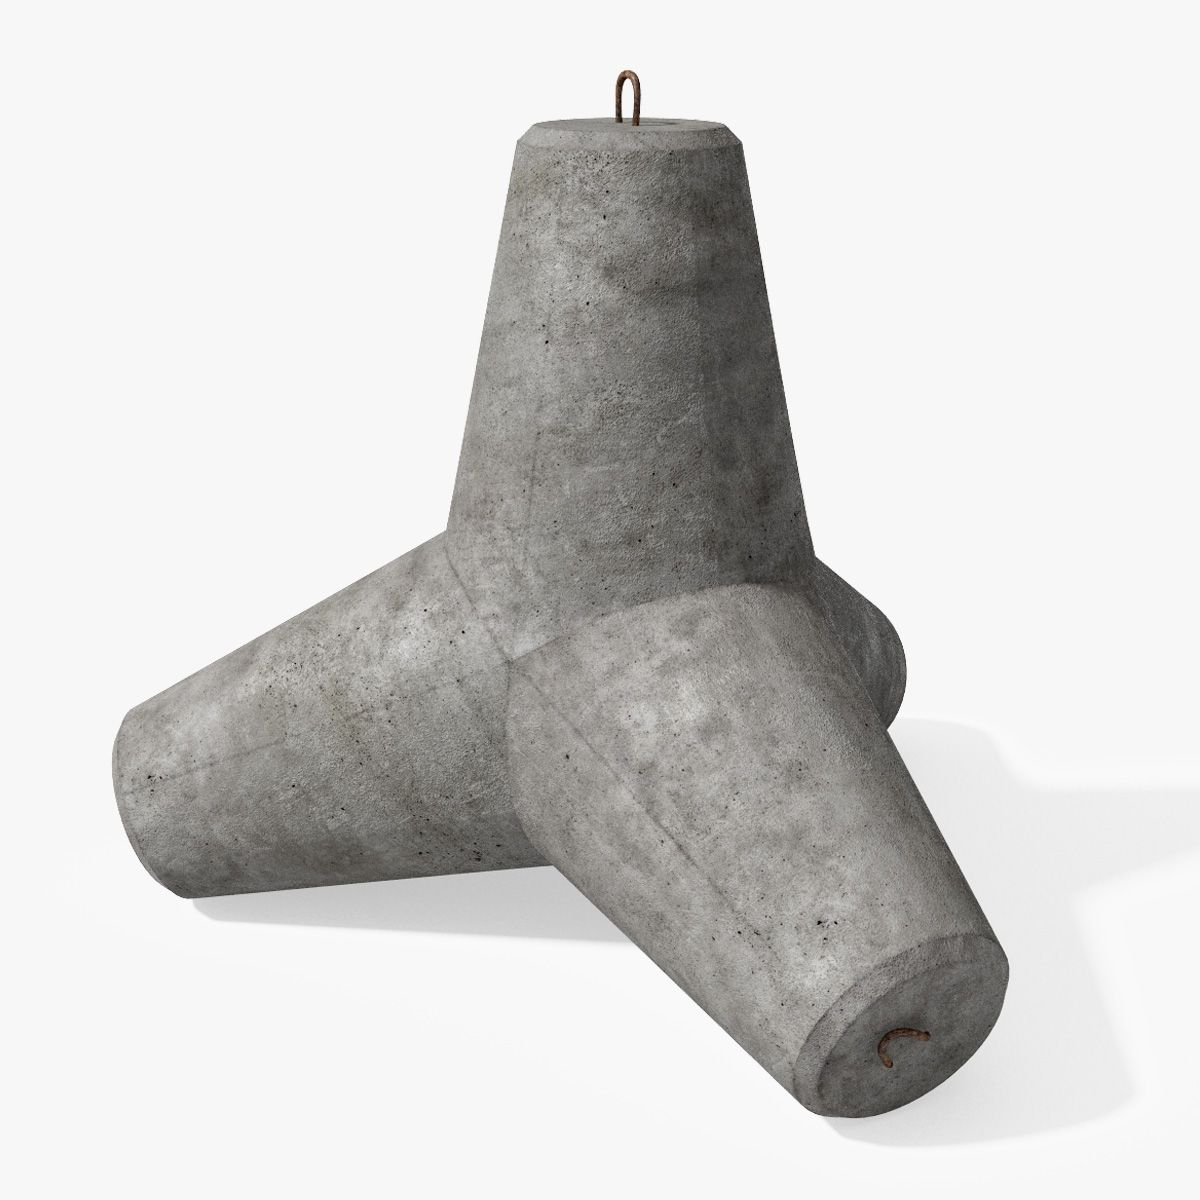
\includegraphics[width=0.30\textwidth]{Tetrapod.png}
  \caption{Concrete Tetrapod used for Coastal Erosion \cite{Free3DTetrapod}.}
  \label{fig:tetrapod_reference}
  \vspace{-1\baselineskip}
\end{wrapfigure}

This studentship will extend the \texttt{MECH0020} numerical framework, supervised by Dr Lama Hamadeh, by advancing from the earlier stream-function--vorticity formulation toward a benchmark tsunami model based on the nonlinear Shallow Water Equations \cite{Bandyopadhyay2021}. Inspired by tetrapods, \smartref{fig:tetrapod_reference}, and related coastal armour units used for wave-energy dissipation and coastal protection, the project will couple a validated large-scale hydrodynamic simulation to a local three-dimensional tsunami--structure interaction model in order to iteratively generate and refine barrier geometries that reduce tsunami energy transmission and structural loading \cite{Dentale2014,Natakusumah2024,Fujima2002,Takase2016,Tozato2022}. The 11 March 2011 T\={o}hoku tsunami will serve as the primary benchmark case study, on two accounts the first being high-quality observational data are available for validation \cite{NCEITohokuEvent,Goto2012} and second is the Sanriku/Tohoku coastline is one of the most historically tsunami-vulnerable regions in Japan, having experienced major destructive events such as the 1896 and 1933 Sanriku tsunamis, while the 2011 event itself produced extreme run-up along the same coast \cite{Fujii2011,Satake2014,Goto2012}.

\vspace{-4mm}
\subsection{Phase I: Benchmark Tsunami Setup and Data Acquisition}\label{sec:phase_i_benchmark_tsunami_setup_and_data_acquisition}
\vspace{-3mm}

The first phase will establish the baseline tsunami simulation by coupling an Okada-type coseismic seabed deformation source with a three-dimensional free-surface hydrodynamic model over realistic bathymetry and topography \cite{Okada1985}, schematics shown in Figures [\ref{fig:Japan},\ref{fig:Wave}]. The model will be validated against published observations of arrival time, peak amplitude, and run-up or inundation extent for the 2011 event \cite{NCEITohokuEvent,Goto2012}. A section immediately upstream of the barrier location will then be used to extract and store the pre-impact boundary histories required for the optimisation stage, so that subsequent candidate geometries can be evaluated in a local three-dimensional tsunami--structure interaction domain without repeating the full-domain simulation \cite{Fujima2002,Takase2016,Tozato2022}.

\vspace{-4mm}
\subsection{Phase II: Machine-Learning-Guided Geometry Optimisation}\label{sec:phase_ii_machine_learning_guided_geometry_optimisation}
\vspace{-3mm}

The second phase will form the core optimisation loop by iteratively refining an initial barrier geometry under simulated tsunami loading. Boundary histories from the baseline tsunami simulation will drive a local three-dimensional tsunami--structure interaction model, allowing candidate designs to be evaluated efficiently while retaining three-dimensional hydrodynamic fidelity. Performance will be assessed through transmitted-wave reduction, attenuation of momentum flux, and reduced load intensity behind the barrier \cite{Dentale2014,Fujima2002,Takase2016,Tozato2022}. The parametrised geometry will then be updated through evolutionary mutation, crossover, and sensitivity-guided local transformations, while the resulting data train a convolutional-neural-network surrogate to guide the search until the prescribed convergence criteria are satisfied \cite{Starodubcev2022,Sidorenko2024}.

\vspace{-4mm}
\subsection{Phase III: Structural Verification and Final Validation}\label{sec:phase_iii_structural_verification_and_final_validation}
\vspace{-3mm}

The final phase will assess the structural viability of the optimised barrier geometry by transferring the shortlisted design into \texttt{ANSYS} or \texttt{ABAQUS} and applying hydrodynamic outputs from the tsunami simulations as equivalent pressures or distributed loads. This stage will evaluate stress distributions, deformation patterns, and structural energy absorption, thereby verifying whether the design remains effective from both hydrodynamic and structural perspectives \cite{Guler2018}. A comparable verification may also be carried out for the reference tetrapod geometry in order to compare structural response and overall performance, and to assess how geometries developed for wave-energy dispersion in coastal erosion protection differ from those optimised for tsunami damping.

\clearpage
\printbibliography
\clearpage
\section*{\centering Appendix}
\begin{figure}[h!]
  \centering
  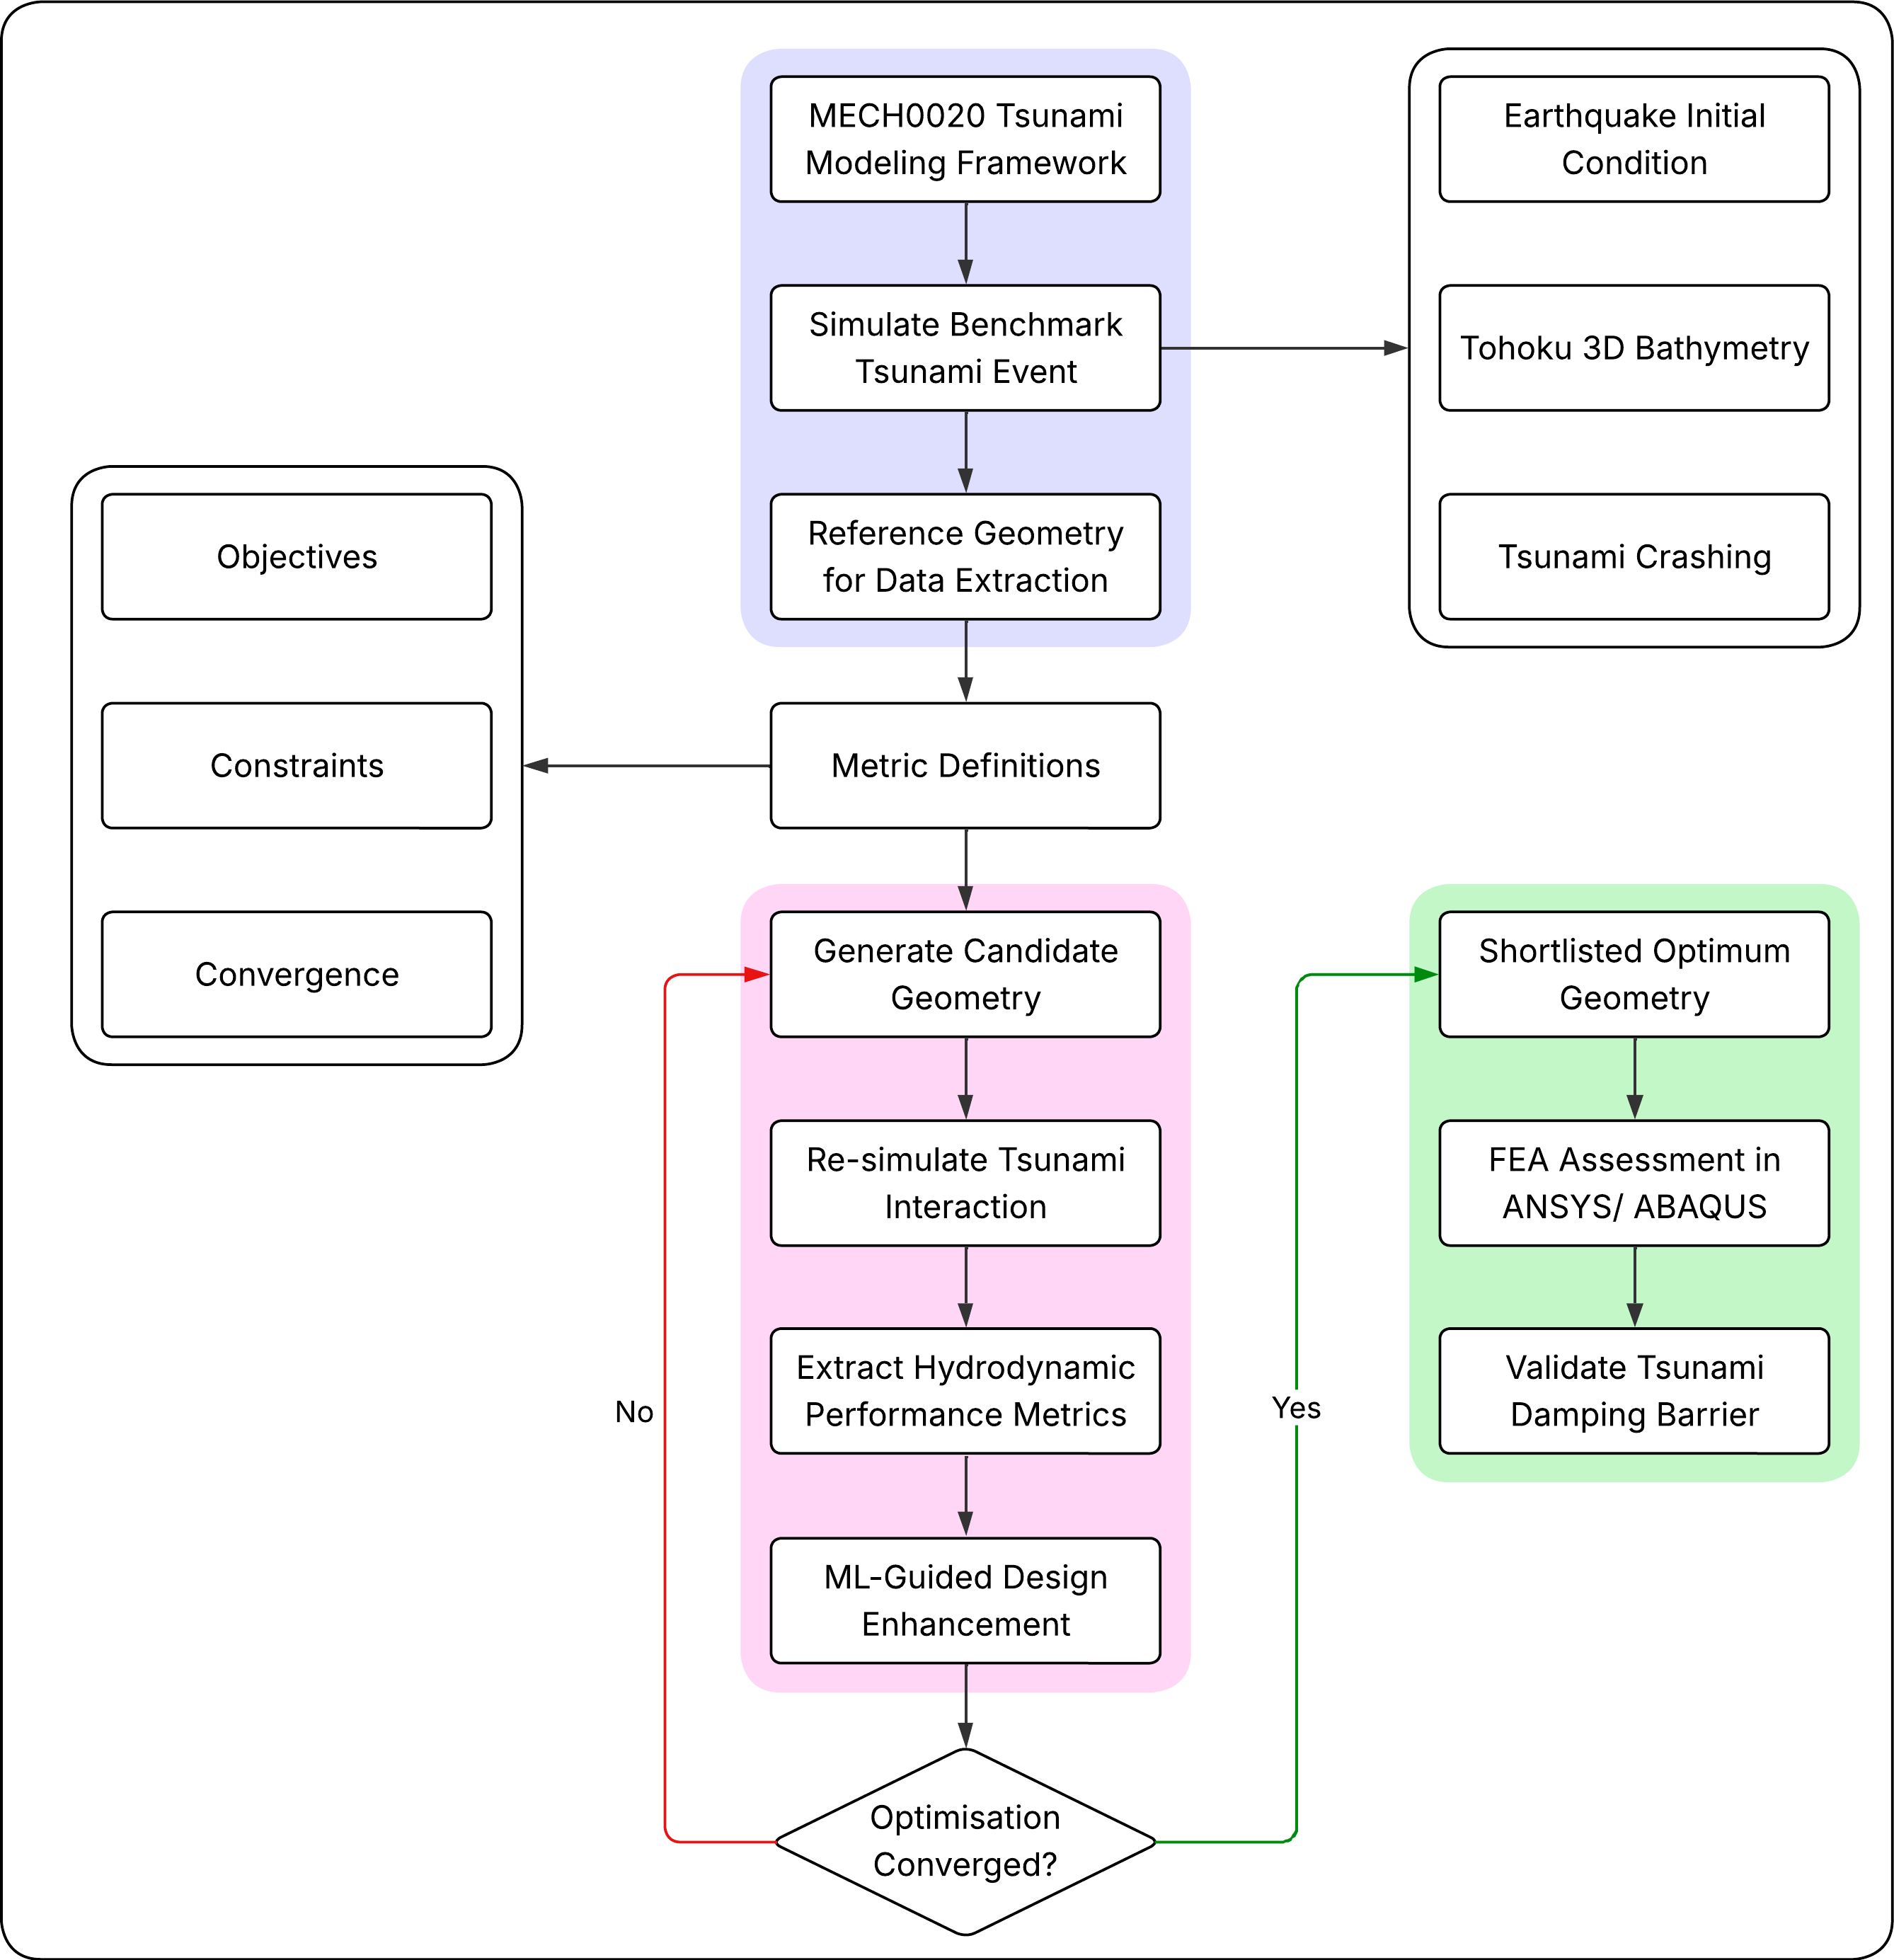
\includegraphics[width=0.8\textwidth]{Studentship Flow.png}
  \caption{Flow chart of the proposed tsunami barrier optimisation framework, with the three principal phases highlighted. Phase I, \textit{Benchmark Tsunami Setup and Data Acquisition}, defines the tsunami scenario and extracts reference hydrodynamic data. Phase II, \textit{Machine-Learning-Guided Geometry Optimisation}, forms the main iterative design loop in which candidate geometries are generated, resimulated, evaluated, and refined until convergence. Phase III, \textit{Structural Verification and Final Validation}, transfers the shortlisted optimum geometry to \texttt{ANSYS}/\texttt{ABAQUS} for structural assessment and final validation. The objective, constraint, and convergence blocks are shown as governing inputs to the optimisation stage.}
  \label{fig:Flowchart}
\end{figure}

\begin{figure}[h!]
  \centering
  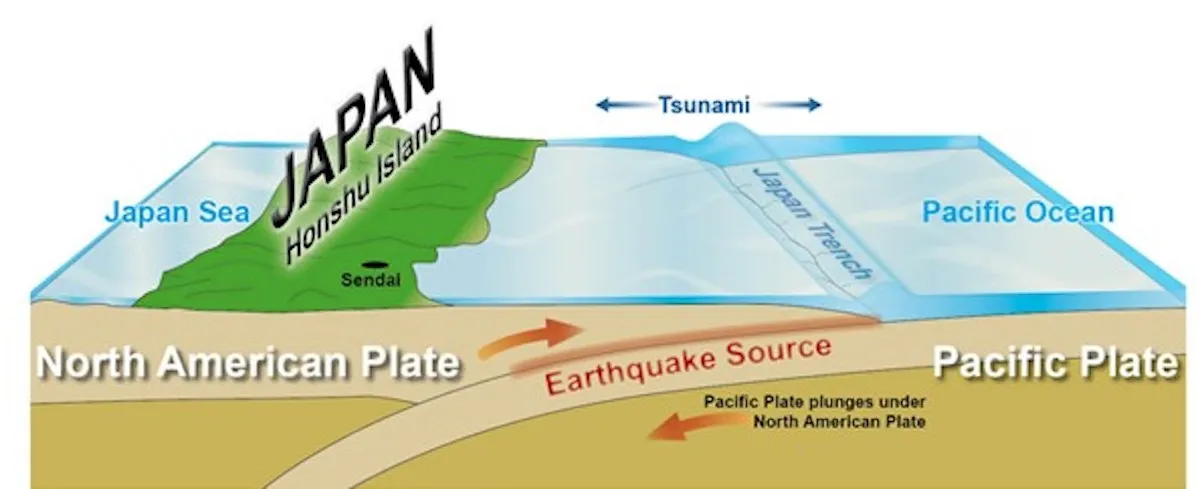
\includegraphics[width=\textwidth]{Japan.png}
  \caption{Schematic illustration of the tectonic setting responsible for the 2011 T\={o}hoku earthquake and tsunami, showing subduction of the Pacific Plate beneath northeastern Honshu and the associated offshore tsunami source region \cite{Foster2021}.}
  \label{fig:Japan}
\end{figure}

\begin{figure}[h!]
  \centering
  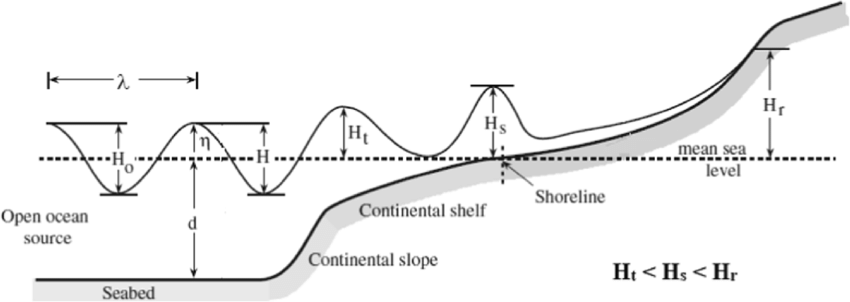
\includegraphics[width=\textwidth]{Tsunami Wave Diagram.png}\caption{Schematic evolution of tsunami wave height from the open ocean to the shoreline, showing the increase in wave elevation and eventual run-up as the wave propagates across the continental slope and shelf toward land\cite{Bandyopadhyay2021}.}
  \label{fig:Wave}
\end{figure}

\end{document}

%                      .-.
%                     (o o)      SCIENCE OWL
%                     | O \      (guardian of rigor)
%                      \   \
%                       `~~~'
%                 .-------------------.
%                 |  NO FABRICATION   |
%                 |  + CLEAR ASSUMES  |
%                 |  + CLEAN LATEX    |
%                 '-------------------'
%            __        __        __        __
%         __/  \__  __/  \__  __/  \__  __/  \__
%        /  RULES  \/  FLOW  \/  MATH  \/  CODE  \
%        \__    __/\__    __/\__    __/\__    __/
%           \__/      \__/      \__/      \__/
%
%                \  |  /        \  |  /
%                 \ | /          \ | /
%              ---- * ----    ---- * ----
%                 / | \          / | \
%                /  |  \        /  |  \
% 
%  \ _^ /   ,^,  % %  \ _^ /   ,^,   % % \ _^ /   ,^,    % %\ _^ /   ,^,
%  \>@@</   ((  % %   \>@@</   ((   % %  \>@@</   ((    % % \>@@</   ((
%   (..)    );)=====   (..)    );) =====  (..)    );)  ===== (..)    );)
%    vv\^^^^ / |   |=   vv\^^^^ /  |   |=  vv\^^^^ /   |   |= vv\^^^^ /
%   /==  ))) ) |   |/  /==  ))) )  |   |/ /==  ))) )   |   |//==  ))) )
%  ( ==/ )=< \ \___/  ( ==/ )=< \  \___/ ( ==/ )=< \   \___/( ==/ )=< \
% {{{)=(}}}(_}}}     {{{)=(}}}(_}}}     {{{)=(}}}(_}}}     {{{)=(}}}(_{{{


%                 %%%;       *                      *
%    |  %%%;     %%%~%%%;               .                     .     *
%  # |__/__%%%____/_/~%;%                           .
%      ___%%;______%%;%          .            *            *
% " " /~ %-//  \ \__%#%%_-%%;`
%    |  ~%-/_%` \ \_/%%#%%`                                            .
% #  | %%%#%     \__/%%#%%;%`,
%   "| ;%%%;`                              *                  .
%    |                            *                  (
% | #|            *        .                                          .
%   ||         .                        . .        .
%    |                .                ` ' `               *
% #  |                             .'''. ' .'''.                   *
%   "|  *           .                .. ' ' ..      .
% '  |                         *    '  '.'.'  '              .
%    |                              .'''.'.'''.
%  " |       .----------.          ' .''.'.''. '
%    |       |__________|            . . : . .
%    |_{}_{}/|__________|\{}_{}_{} _'___':'___'_ {}_{}_{}_{}_{}_{}_{}_{}
% ' #| || ||/____________\|| || ||(_____________)|| || || || || || || ||
% lc'\""""""||          ||""""""""""""(     )"""""""""""""""""""""""""""
% """""     |            |            _)   (_             .^-^.  ~""~
%                          ~""~      (_______)~~"""~~     '._.'
%     ~~""~~                     ~""~                     .' '.
%                                                         '.,.'
%                                                            `'`'